\documentclass[tikz,border=10pt]{standalone}
\begin{document}
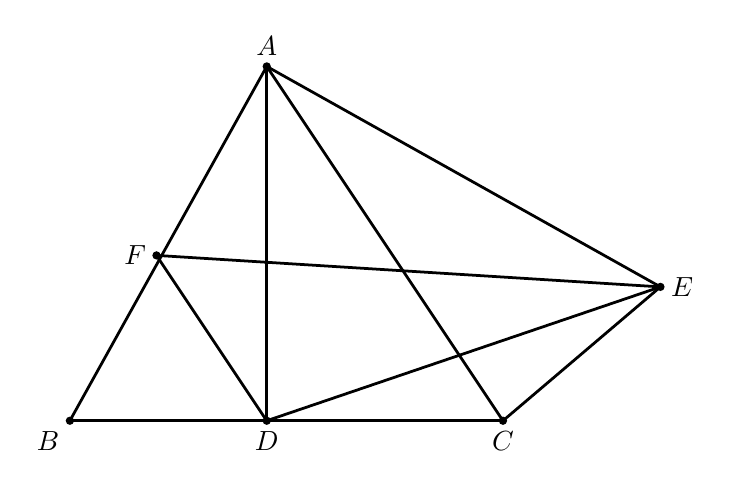
\begin{tikzpicture}[line width=1pt]
\coordinate (A) at (2.5,4.5);
\coordinate (B) at (0,0);
\coordinate (C) at (5.5,0);
\coordinate (D) at (2.5,0);
\coordinate (E) at (7.5,1.7);
\coordinate (F) at (1.1,2.1);

\draw (B) -- (C);
\draw (A) -- (B);
\draw (A) -- (C);
\draw (A) -- (D);
\draw (A) -- (E);
\draw (F) -- (D);
\draw (F) -- (E);
\draw (D) -- (E);
\draw (C) -- (E);

\foreach \p/\pos in {A/above,B/below left,C/below,D/below,E/right,F/left}
  \node at (\p) [\pos] {$\p$};
\foreach \p in {A,B,C,D,E,F}
  \fill (\p) circle (1.5pt);
\end{tikzpicture}
\end{document}
